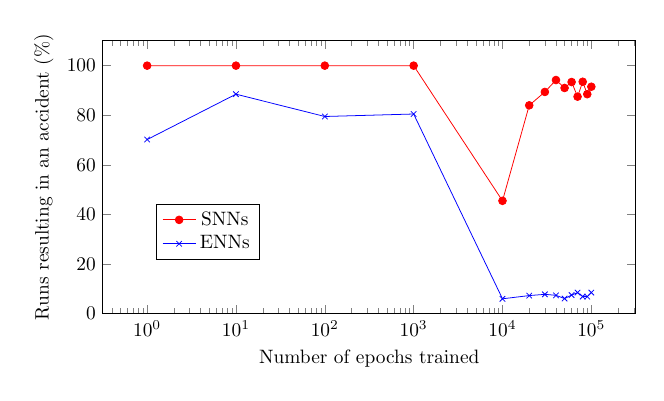
\begin{tikzpicture}[scale=0.7]
\begin{semilogxaxis}[
xlabel={Number of epochs trained},
ylabel={Runs resulting in an accident (\%)},
x=0.7cm,
y=0.45mm, 
ymin=0,
legend style={at={(0.1,0.3)},anchor=west}]

\addplot[color=red,mark=*] coordinates {
	(0, 100)
	(1, 100)
	(10, 100)
	(100, 100)
	(1000, 100)
	(10000, 45.5)
	(20000, 84.0)
	(30000, 89.4)
	(40000, 94.2)
	(50000, 91.0)
	(60000, 93.4)
	(70000, 87.5)
	(80000, 93.5)
	(90000, 88.5)
	(100000, 91.5)
};

\addplot[color=blue,mark=x] coordinates {
	(0, 75.7)
	(1, 70.2)
	(10, 88.5)
	(100, 79.5)
	(1000, 80.5)
	(10000, 6.0)  
	(20000, 7.3)
	(30000, 7.8)
	(40000, 7.4)
	(50000, 6.1)
	(60000, 7.5)
	(70000, 8.5)
	(80000, 6.9)
	(90000, 6.9) 
	(100000, 8.5) 
};

\legend{SNNs, ENNs}
\end{semilogxaxis}%
\end{tikzpicture}%